\documentclass{standalone}
\usepackage{tikz}
\usetikzlibrary{patterns, positioning}
\usepackage[sfdefault]{ClearSans} %% option 'sfdefault' activates Clear Sans as the default text font
\usepackage[T1]{fontenc}

\begin{document}
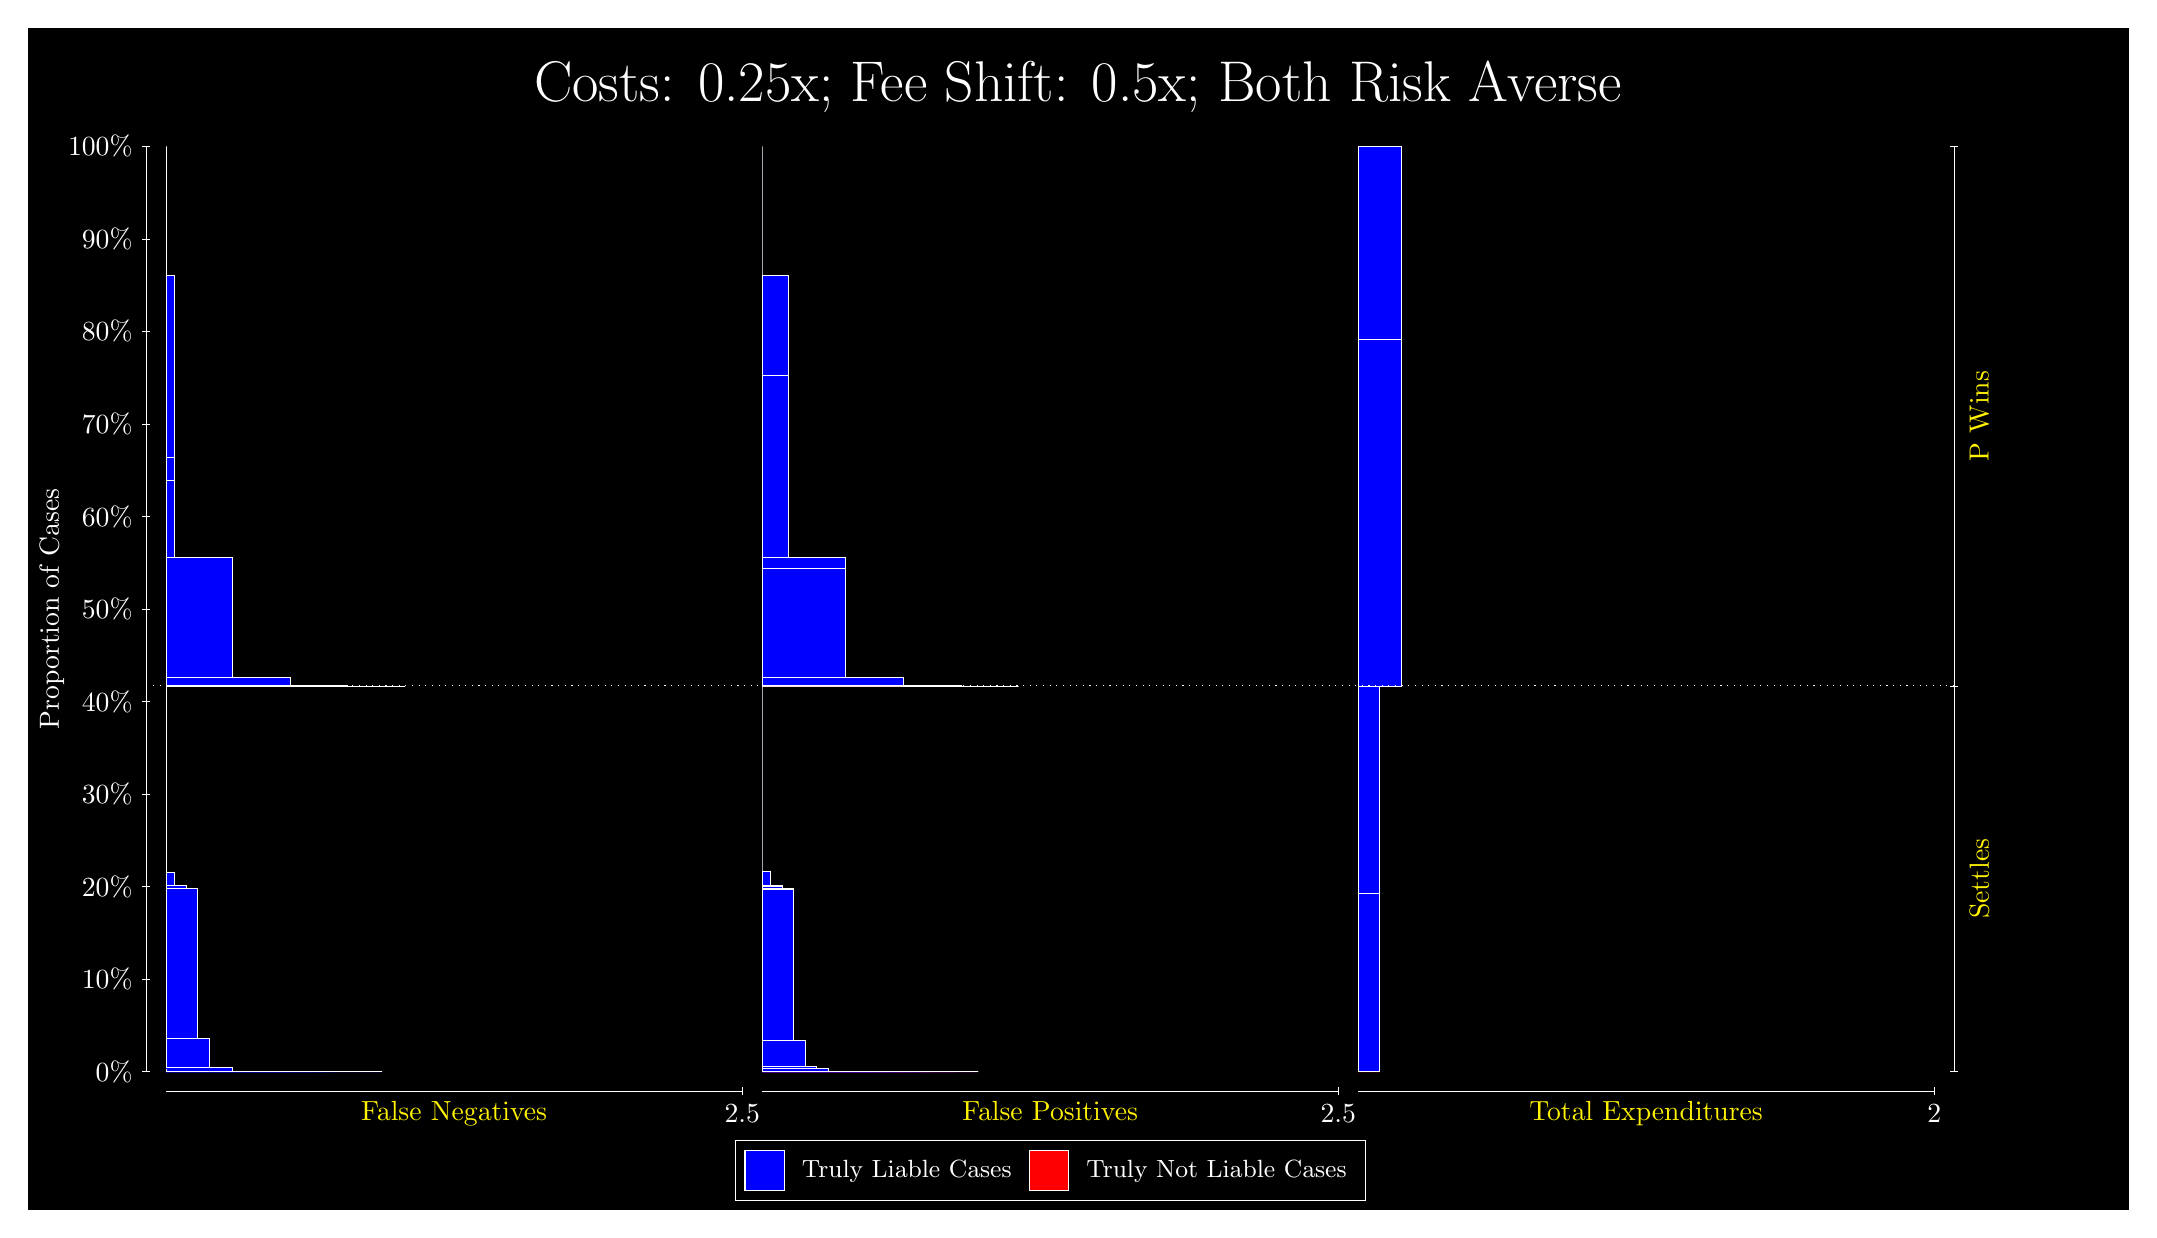
\begin{tikzpicture}
\draw[fill=black] (0,0) rectangle (26.667,15);
\draw[text=white] (0,13.5) rectangle (26.667,15) node[midway] {\huge Costs: 0.25x; Fee Shift: 0.5x; Both Risk Averse};
\draw[white, very thin] (1.5,1.75) -- (1.5,13.5);
\node[rotate=90, text=white, anchor=center] at (0.3, 7.625) {Proportion of Cases};
\draw[white, very thin] (1.45,1.75) -- (1.55,1.75);
\node[text=white, anchor=east] at (1.45, 1.75) {0\%};
\draw[white, very thin] (1.45,2.925) -- (1.55,2.925);
\node[text=white, anchor=east] at (1.45, 2.925) {10\%};
\draw[white, very thin] (1.45,4.1) -- (1.55,4.1);
\node[text=white, anchor=east] at (1.45, 4.1) {20\%};
\draw[white, very thin] (1.45,5.275) -- (1.55,5.275);
\node[text=white, anchor=east] at (1.45, 5.275) {30\%};
\draw[white, very thin] (1.45,6.45) -- (1.55,6.45);
\node[text=white, anchor=east] at (1.45, 6.45) {40\%};
\draw[white, very thin] (1.45,7.625) -- (1.55,7.625);
\node[text=white, anchor=east] at (1.45, 7.625) {50\%};
\draw[white, very thin] (1.45,8.8) -- (1.55,8.8);
\node[text=white, anchor=east] at (1.45, 8.8) {60\%};
\draw[white, very thin] (1.45,9.975) -- (1.55,9.975);
\node[text=white, anchor=east] at (1.45, 9.975) {70\%};
\draw[white, very thin] (1.45,11.15) -- (1.55,11.15);
\node[text=white, anchor=east] at (1.45, 11.15) {80\%};
\draw[white, very thin] (1.45,12.325) -- (1.55,12.325);
\node[text=white, anchor=east] at (1.45, 12.325) {90\%};
\draw[white, very thin] (1.45,13.5) -- (1.55,13.5);
\node[text=white, anchor=east] at (1.45, 13.5) {100\%};

\draw[white, very thin] (24.457,1.75) -- (24.457,13.5);
\draw[white, very thin] (24.407,1.75) -- (24.507,1.75);
\node[anchor=west] at (24.407, 1.75) {};
\draw[white, very thin] (24.407,6.6484) -- (24.507,6.6484);
\node[anchor=west] at (24.407, 6.6484) {};
\draw[white, very thin] (24.407,13.5) -- (24.507,13.5);
\node[anchor=west] at (24.407, 13.5) {};

\draw[white, very thin, fill=blue] (1.75,1.75) rectangle (4.4946,1.75);
\draw[white, very thin, fill=blue] (1.75,1.75) rectangle (3.9091,1.75);
\draw[white, very thin, fill=blue] (1.75,1.75) rectangle (3.7627,1.75);
\draw[white, very thin, fill=blue] (1.75,1.75) rectangle (3.6163,1.75);
\draw[white, very thin, fill=blue] (1.75,1.75) rectangle (3.3236,1.7501);
\draw[white, very thin, fill=blue] (1.75,1.7501) rectangle (3.1772,1.7501);
\draw[white, very thin, fill=blue] (1.75,1.7501) rectangle (3.0308,1.7524);
\draw[white, very thin, fill=blue] (1.75,1.7524) rectangle (2.8844,1.7524);
\draw[white, very thin, fill=blue] (1.75,1.7524) rectangle (2.738,1.7533);
\draw[white, very thin, fill=blue] (1.75,1.7533) rectangle (2.5917,1.7987);
\draw[white, very thin, fill=blue] (1.75,1.7987) rectangle (2.4453,1.7996);
\draw[white, very thin, fill=blue] (1.75,1.7996) rectangle (2.4453,1.8004);
\draw[white, very thin, fill=blue] (1.75,1.8004) rectangle (2.2989,2.1719);
\draw[white, very thin, fill=blue] (1.75,2.1719) rectangle (2.1525,2.172);
\draw[white, very thin, fill=blue] (1.75,2.172) rectangle (2.1525,4.0771);
\draw[white, very thin, fill=blue] (1.75,4.0771) rectangle (2.0062,4.1091);
\draw[white, very thin, fill=blue] (1.75,4.1091) rectangle (1.8598,4.2857);
\draw[white, very thin, fill=red] (1.75,4.2857) rectangle (1.75,4.2857);
\draw[white, very thin, fill=blue] (1.75,4.2857) rectangle (1.75,6.6484);
\draw[white, very thin, fill=blue] (1.75,6.6484) rectangle (4.7873,6.6484);
\draw[white, very thin, fill=blue] (1.75,6.6484) rectangle (4.0554,6.6495);
\draw[white, very thin, fill=blue] (1.75,6.6495) rectangle (3.3236,6.7537);
\draw[white, very thin, fill=blue] (1.75,6.7537) rectangle (2.5917,8.2813);
\draw[white, very thin, fill=blue] (1.75,8.2813) rectangle (1.8598,9.2622);
\draw[white, very thin, fill=blue] (1.75,9.2622) rectangle (1.8598,9.5556);
\draw[white, very thin, fill=blue] (1.75,9.5556) rectangle (1.8598,11.866);
\draw[white, very thin, fill=red] (1.75,11.866) rectangle (1.75,11.866);
\draw[white, very thin, fill=blue] (1.75,11.866) rectangle (1.75,13.5);
\draw[white, very thin, fill=red] (9.3189,1.75) rectangle (12.063,1.75);
\draw[white, very thin, fill=blue] (9.3189,1.75) rectangle (12.063,1.75);
\draw[white, very thin, fill=red] (9.3189,1.75) rectangle (11.771,1.75);
\draw[white, very thin, fill=blue] (9.3189,1.75) rectangle (11.771,1.75);
\draw[white, very thin, fill=red] (9.3189,1.75) rectangle (11.478,1.75);
\draw[white, very thin, fill=blue] (9.3189,1.75) rectangle (11.478,1.75);
\draw[white, very thin, fill=blue] (9.3189,1.75) rectangle (11.332,1.75);
\draw[white, very thin, fill=red] (9.3189,1.75) rectangle (11.185,1.75);
\draw[white, very thin, fill=blue] (9.3189,1.75) rectangle (11.185,1.75);
\draw[white, very thin, fill=blue] (9.3189,1.75) rectangle (11.039,1.75);
\draw[white, very thin, fill=red] (9.3189,1.75) rectangle (10.892,1.75);
\draw[white, very thin, fill=blue] (9.3189,1.75) rectangle (10.892,1.7501);
\draw[white, very thin, fill=blue] (9.3189,1.7501) rectangle (10.746,1.7502);
\draw[white, very thin, fill=blue] (9.3189,1.7502) rectangle (10.6,1.7518);
\draw[white, very thin, fill=red] (9.3189,1.7518) rectangle (10.6,1.7518);
\draw[white, very thin, fill=blue] (9.3189,1.7518) rectangle (10.6,1.7518);
\draw[white, very thin, fill=blue] (9.3189,1.7518) rectangle (10.453,1.7521);
\draw[white, very thin, fill=blue] (9.3189,1.7521) rectangle (10.307,1.7528);
\draw[white, very thin, fill=red] (9.3189,1.7528) rectangle (10.307,1.7528);
\draw[white, very thin, fill=blue] (9.3189,1.7528) rectangle (10.307,1.7536);
\draw[white, very thin, fill=blue] (9.3189,1.7536) rectangle (10.161,1.7965);
\draw[white, very thin, fill=blue] (9.3189,1.7965) rectangle (10.014,1.8151);
\draw[white, very thin, fill=blue] (9.3189,1.8151) rectangle (9.8678,2.1524);
\draw[white, very thin, fill=blue] (9.3189,2.1524) rectangle (9.8678,2.1525);
\draw[white, very thin, fill=red] (9.3189,2.1525) rectangle (9.7214,2.1525);
\draw[white, very thin, fill=blue] (9.3189,2.1525) rectangle (9.7214,4.0586);
\draw[white, very thin, fill=blue] (9.3189,4.0586) rectangle (9.7214,4.0821);
\draw[white, very thin, fill=blue] (9.3189,4.0821) rectangle (9.575,4.0979);
\draw[white, very thin, fill=blue] (9.3189,4.0979) rectangle (9.575,4.1127);
\draw[white, very thin, fill=blue] (9.3189,4.1127) rectangle (9.4287,4.2893);
\draw[white, very thin, fill=blue] (9.3189,4.2893) rectangle (9.3189,6.6484);
\draw[white, very thin, fill=red] (9.3189,6.6484) rectangle (12.576,6.6484);
\draw[white, very thin, fill=blue] (9.3189,6.6484) rectangle (12.576,6.6484);
\draw[white, very thin, fill=red] (9.3189,6.6484) rectangle (11.844,6.6484);
\draw[white, very thin, fill=blue] (9.3189,6.6484) rectangle (11.844,6.6495);
\draw[white, very thin, fill=red] (9.3189,6.6495) rectangle (11.112,6.6495);
\draw[white, very thin, fill=blue] (9.3189,6.6495) rectangle (11.112,6.7545);
\draw[white, very thin, fill=blue] (9.3189,6.7545) rectangle (10.38,8.146);
\draw[white, very thin, fill=red] (9.3189,8.146) rectangle (10.38,8.146);
\draw[white, very thin, fill=blue] (9.3189,8.146) rectangle (10.38,8.2821);
\draw[white, very thin, fill=blue] (9.3189,8.2821) rectangle (9.6482,10.593);
\draw[white, very thin, fill=red] (9.3189,10.593) rectangle (9.6482,10.593);
\draw[white, very thin, fill=blue] (9.3189,10.593) rectangle (9.6482,11.867);
\draw[white, very thin, fill=blue] (9.3189,11.867) rectangle (9.3189,13.5);
\draw[white, very thin, fill=red] (16.888,1.75) rectangle (17.162,1.75);
\draw[white, very thin, fill=blue] (16.888,1.75) rectangle (17.162,4.0135);
\draw[white, very thin, fill=red] (16.888,4.0135) rectangle (17.162,4.0135);
\draw[white, very thin, fill=blue] (16.888,4.0135) rectangle (17.162,6.6484);
\draw[white, very thin, fill=red] (16.888,6.6484) rectangle (17.437,6.6484);
\draw[white, very thin, fill=blue] (16.888,6.6484) rectangle (17.437,11.053);
\draw[white, very thin, fill=red] (16.888,11.053) rectangle (17.437,11.053);
\draw[white, very thin, fill=blue] (16.888,11.053) rectangle (17.437,13.5);
\draw[white, dotted] (1.5,6.6484) -- (24.457,6.6484);
\draw[white, very thin] (1.75,1.5) -- (9.0689,1.5);
\node[text=yellow, anchor=north] at (5.4094, 1.5) {False Negatives};
\draw[white, very thin] (9.0689,1.45) -- (9.0689,1.55);
\node[text=white, anchor=north] at (9.0689, 1.45) {2.5};

\draw[white, very thin] (9.3189,1.5) -- (16.638,1.5);
\node[text=yellow, anchor=north] at (12.978, 1.5) {False Positives};
\draw[white, very thin] (16.638,1.45) -- (16.638,1.55);
\node[text=white, anchor=north] at (16.638, 1.45) {2.5};

\draw[white, very thin] (16.888,1.5) -- (24.207,1.5);
\node[text=yellow, anchor=north] at (20.547, 1.5) {Total Expenditures};
\draw[white, very thin] (24.207,1.45) -- (24.207,1.55);
\node[text=white, anchor=north] at (24.207, 1.45) {2};

\node[text=yellow, centered, rotate=90] at (24.777, 4.1992) {Settles};
\node[text=yellow, centered, rotate=90] at (24.777, 10.074) {P Wins};

\draw (12.978300999999998,1.5) node[draw=none] (baseCoordinate) {};
\begin{scope}[align=center]
        \matrix[scale=0.5, draw=white, below=0.5cm of baseCoordinate, nodes={draw}, column sep=0.1cm]{
            \node[rectangle, draw, minimum width=0.5cm, minimum height=0.5cm, fill=blue] {}; &
            \node[draw=none, font=\small, text=white] (B) {Truly Liable Cases}; &
            \node[rectangle, draw, minimum width=0.5cm, minimum height=0.5cm, fill=red] {}; &
            \node[draw=none, font=\small, text=white] (B) {Truly Not Liable Cases}; \\
            };
\end{scope}

\end{tikzpicture}
\end{document}